\section{Triggers}
\label{sec:trigger}

In this analysis we use various sets of triggers in order to achieve an optimal selection efficiency. For each dilepton channel ($ee$, $\mu\mu$ and $e\mu$) we take the logical OR
of the dilepton triggers listed in Tab.~\ref{table:triggers} thus combining isolated and non-isolated triggers.
We moreover complement the partially inefficient dilepton triggers by single lepton triggers and remove the overlap between two primary data sets by vetoing events that 
fired a dilepton trigger in the single lepton primary data sets.
Because the e$\mu$ channel is complemented by two single lepton primary data sets, the procedure has two steps: We first add events from the {\verb SingleElectron } primary data set
that fired single electron triggers but failed the double lepton triggers that we use to select events in the {\verb MuonEG } primary data set. We furthermore add events from the
{\verb SingleMuon } primary data set that fired single muon triggers but fired none of the triggers we use to select events in either the {\verb MuonEG } or the {\verb SingleElectron } primary data set.

Table \ref{table:triggers} gives an overview of all triggers used in this analysis.

\begin{table}
  \center
  \scriptsize
  \begin{tabular}{c|l|l}
     channel  & primary dataset & HLT paths\\
     \hline
     $ee$     & DoubleEG        & \verb HLT_Ele23_Ele12_CaloIdL_TrackIdL_IsoVL_DZ \\
              &                 & \verb HLT_Ele17_Ele12_CaloIdL_TrackIdL_IsoVL_DZ \\
              &                 & \verb HLT_DoubleEle33_CaloIdL_GsfTrkIdVL \\
              &                 & \verb HLT_DoubleEle33_CaloIdL_GsfTrkIdVL_MW \\
              & SingleElectron  & \verb HLT_Ele105_CaloIdVT_GsfTrkIdT \\
              &                 & \verb HLT_Ele115_CaloIdVT_GsfTrkIdT \\
     \hline
     $\mu\mu$ & DoubleMuon      & \verb HLT_Mu17_TrkIsoVVL_Mu8_TrkIsoVVL \\
              &                 & \verb HLT_Mu17_TrkIsoVVL_Mu8_TrkIsoVVL_DZ \\
              &                 & \verb HLT_Mu17_TrkIsoVVL_TkMu8_TrkIsoVVL \\
              &                 & \verb HLT_Mu17_TrkIsoVVL_TkMu8_TrkIsoVVL_DZ \\
              &                 & \verb HLT_Mu30_TkMu11 \\
              & SingleMuon      & \verb HLT_Mu50 \\
              &                 & \verb HLT_TkMu50 \\
              &                 & \verb HLT_Mu45_eta2p1 \\
     \hline
     $e\mu$   & MuonEG          & \verb HLT_Mu23_TrkIsoVVL_Ele12_CaloIdL_TrackIdL_IsoVL \\
              &                 & \verb HLT_Mu17_TrkIsoVVL_Ele12_CaloIdL_TrackIdL_IsoVL \\
              &                 & \verb HLT_Mu8_TrkIsoVVL_Ele23_CaloIdL_TrackIdL_IsoVL \\
              &                 & \verb HLT_Mu8_TrkIsoVVL_Ele17_CaloIdL_TrackIdL_IsoVL \\
              &                 & \verb HLT_Mu30_Ele30_CaloIdL_GsfTrkIdVL \\
              & SingleElectron  & \verb HLT_Ele105_CaloIdVT_GsfTrkIdT \\
              &                 & \verb HLT_Ele115_CaloIdVT_GsfTrkIdT \\
              & SingleMuon      & \verb HLT_Mu50 \\
              &                 & \verb HLT_TkMu50 \\
              &                 & \verb HLT_Mu45_eta2p1 \\
  \end{tabular}
  \caption{Summary of HLT triggers grouped by channel and primary dataset. }
  \label{table:triggers}
\end{table}

%\subsection{Trigger efficiencies}

% figures from http://schoef.web.cern.ch/schoef/pngEff/
\begin{figure}
  \centering
  %\subfloat[only isolated double-lepton triggers][only isolated \\ double-lepton triggers]{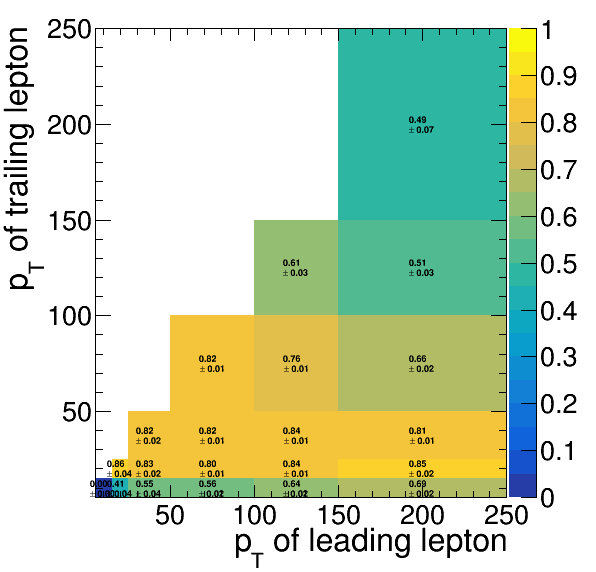
\includegraphics[width=0.5\textwidth]{figures/trigger/HLT_mumu_pt1_pt2_highEta1_NOAddTrig.png}}
  %\subfloat[including non-isolated double-lepton triggers][including non-isolated \\ double-lepton triggers]{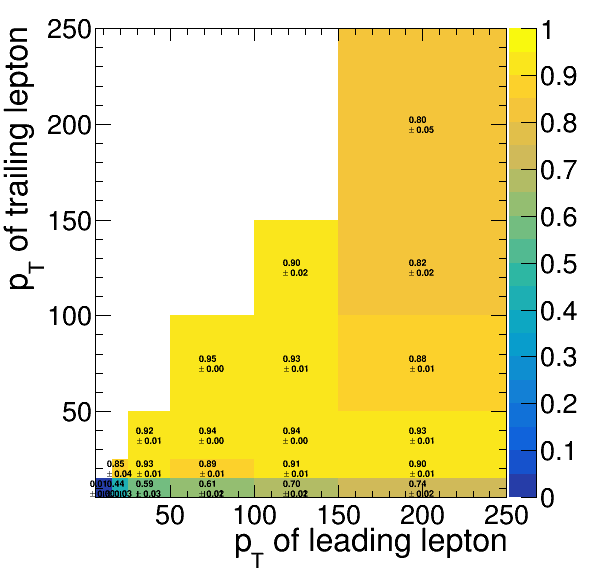
\includegraphics[width=0.5\textwidth]{figures/trigger/HLT_mumu_pt1_pt2_highEta1_DoubleLepTrigOR.png}}\\
  %\subfloat[including single-lepton triggers][including \\ single-lepton triggers]{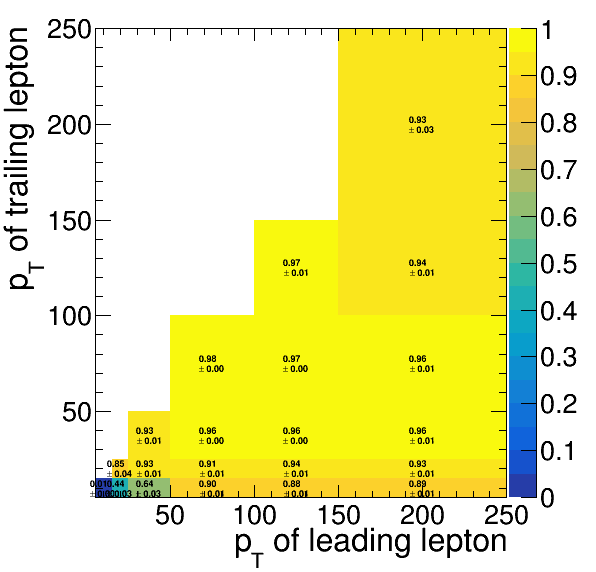
\includegraphics[width=0.5\textwidth]{figures/trigger/HLT_mumu_pt1_pt2_highEta1_AllTriggersInOR.png}}
  \subfloat[only isolated double-lepton triggers][only isolated \\ double-lepton triggers]{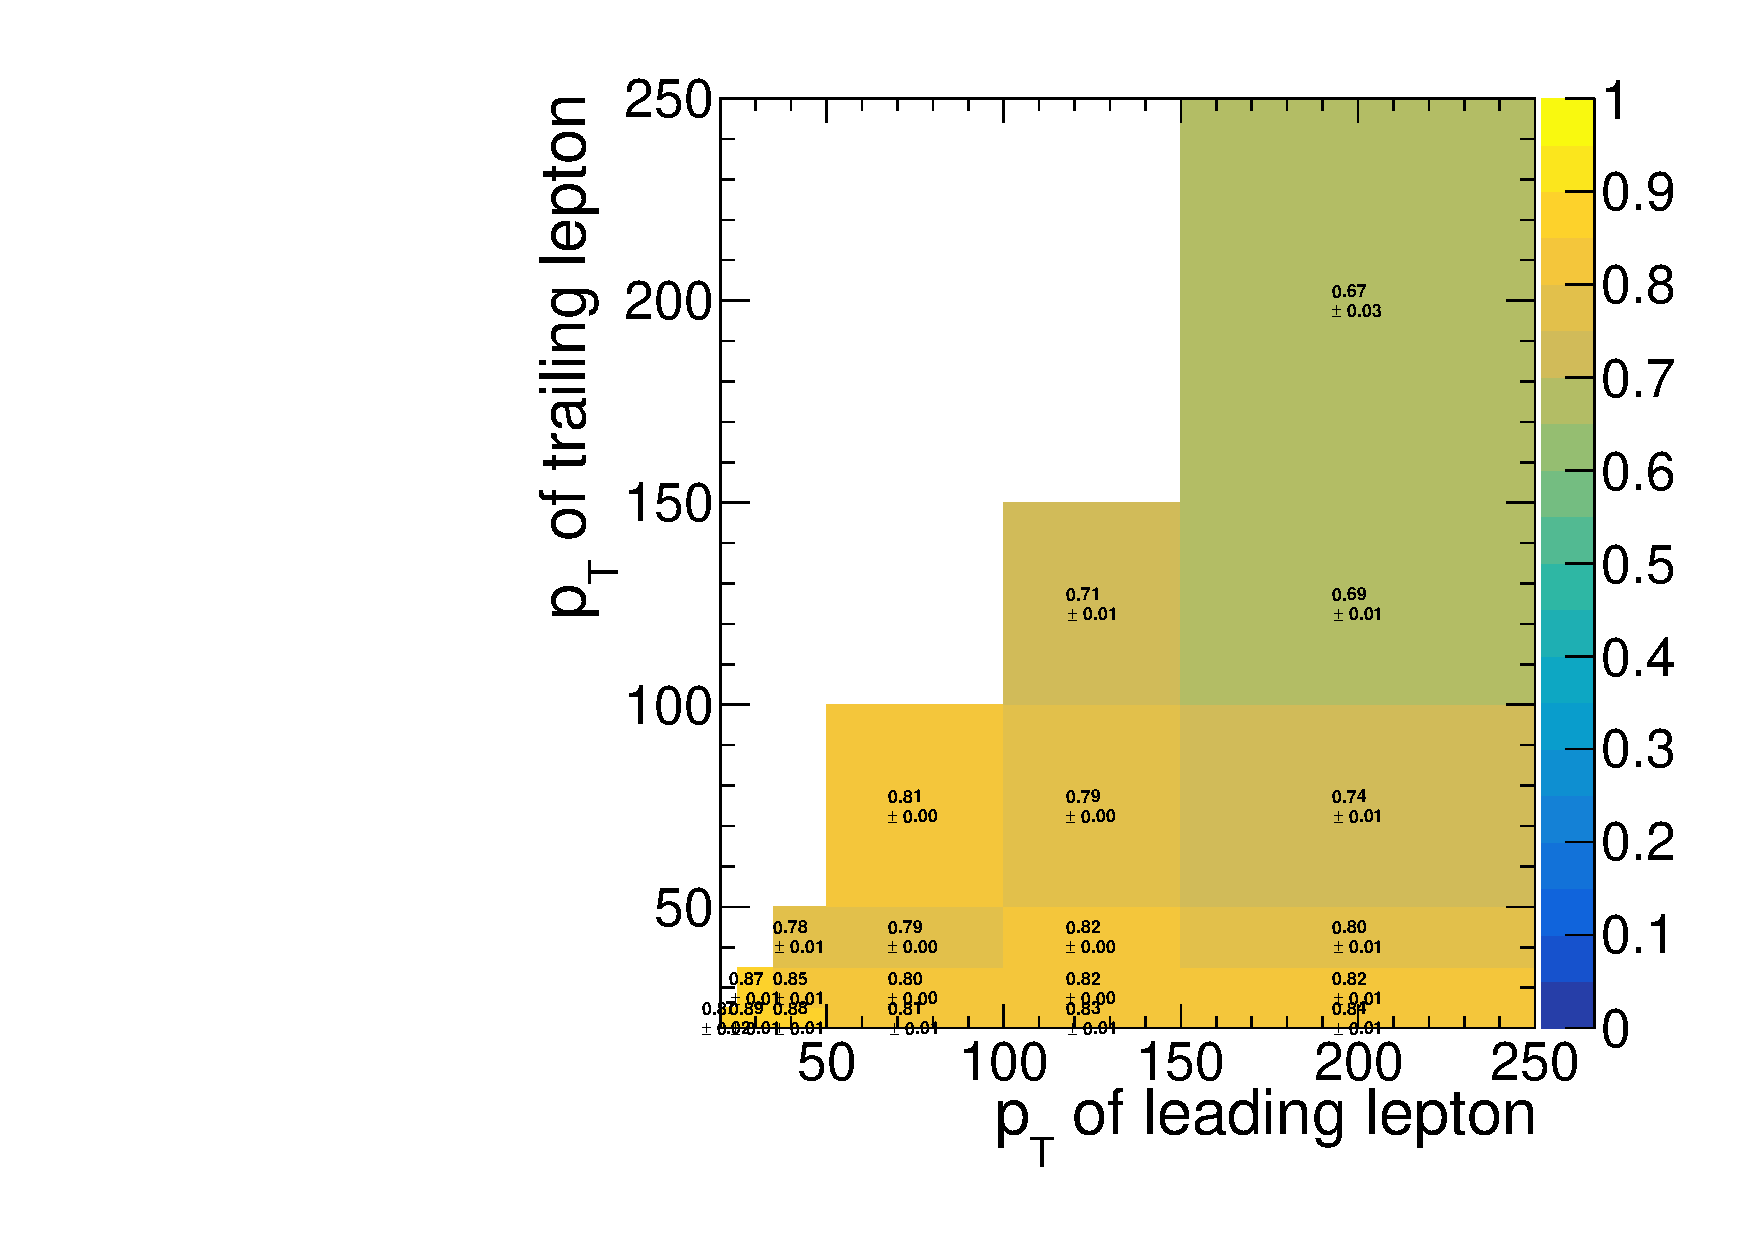
\includegraphics[width=0.5\textwidth]{figures/trigger/HLT_mumuIso_pt1_pt2_highEta1_veryCoarse_BCDEF.pdf}}
  \subfloat[including non-isolated double-lepton triggers][including non-isolated \\ double-lepton triggers]{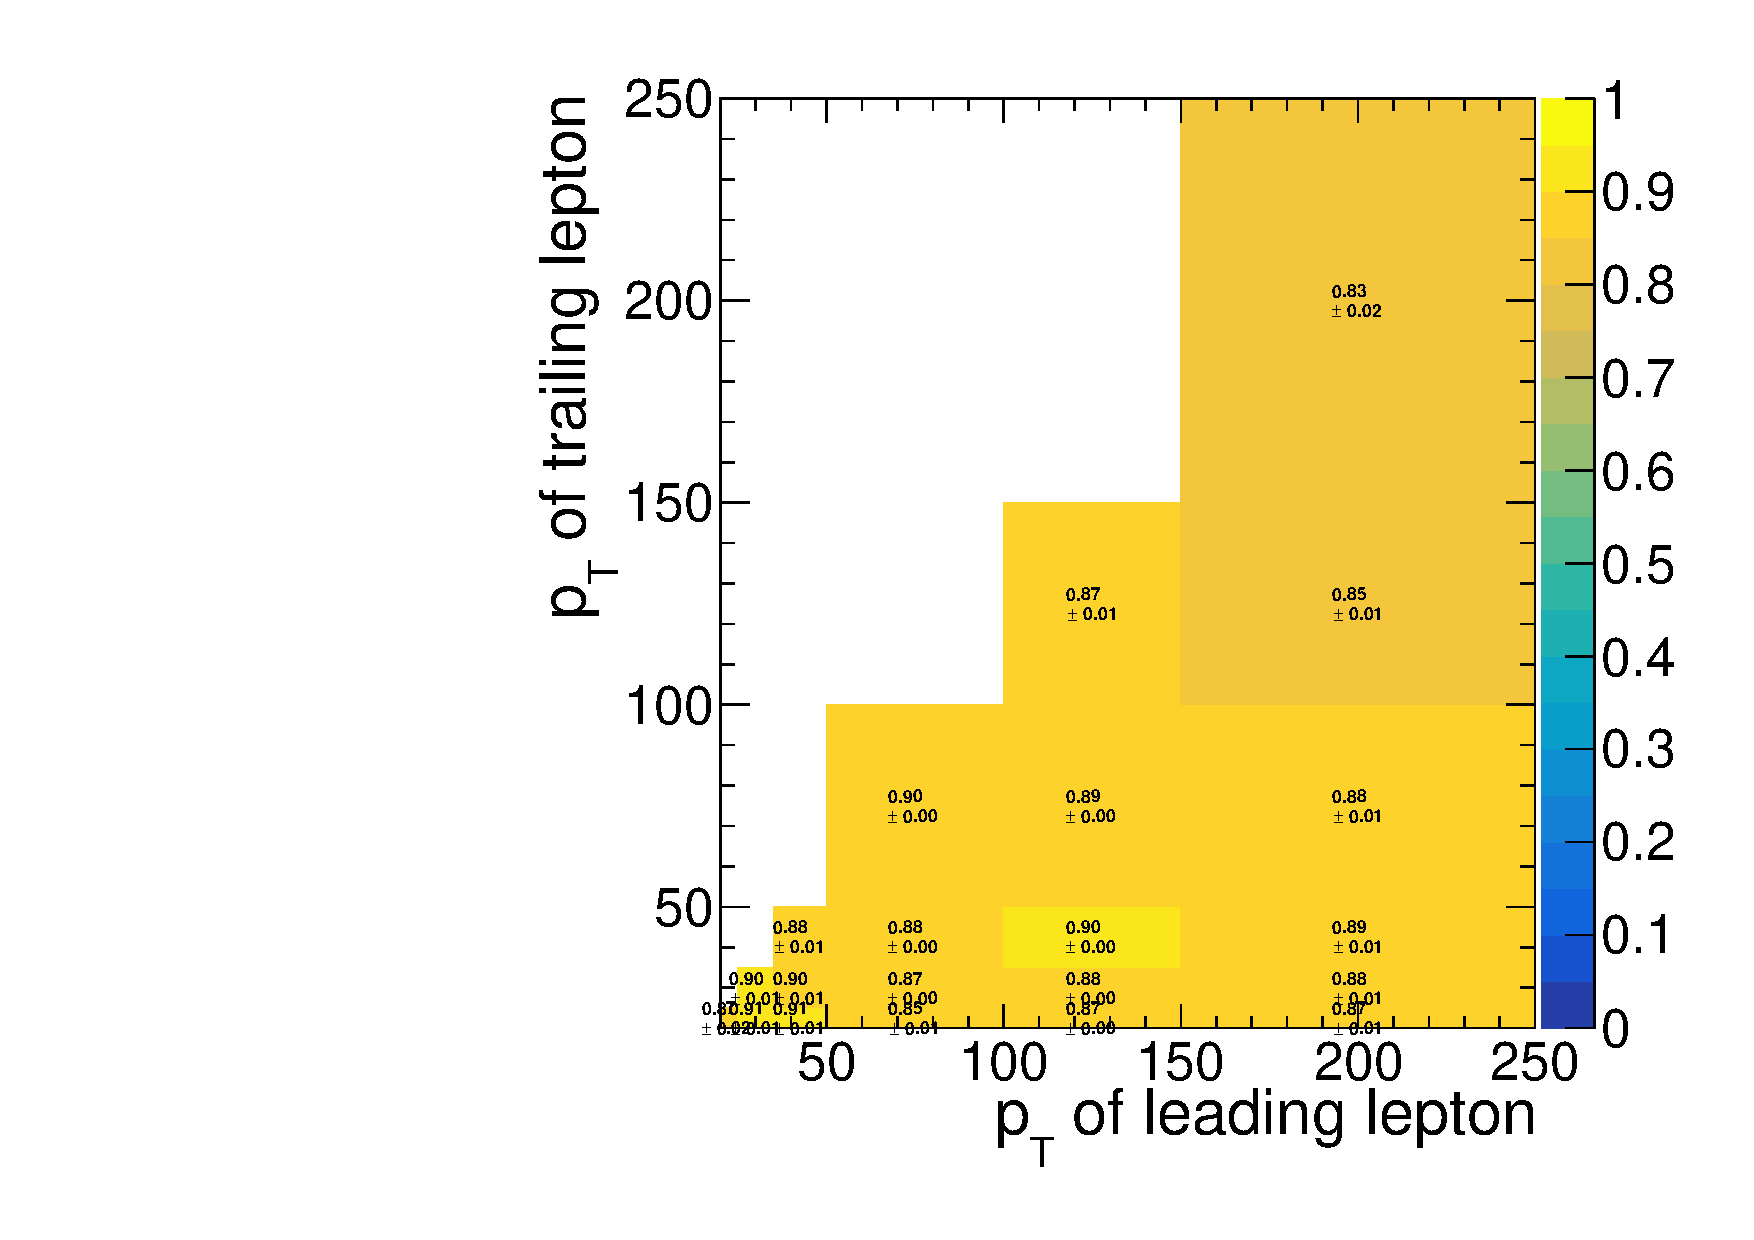
\includegraphics[width=0.5\textwidth]{figures/trigger/HLT_mumuIso_OR_HLT_mumuNoiso_pt1_pt2_highEta1_veryCoarse_BCDEF.pdf}}\\
  \subfloat[including single-lepton triggers][including \\ single-lepton triggers]{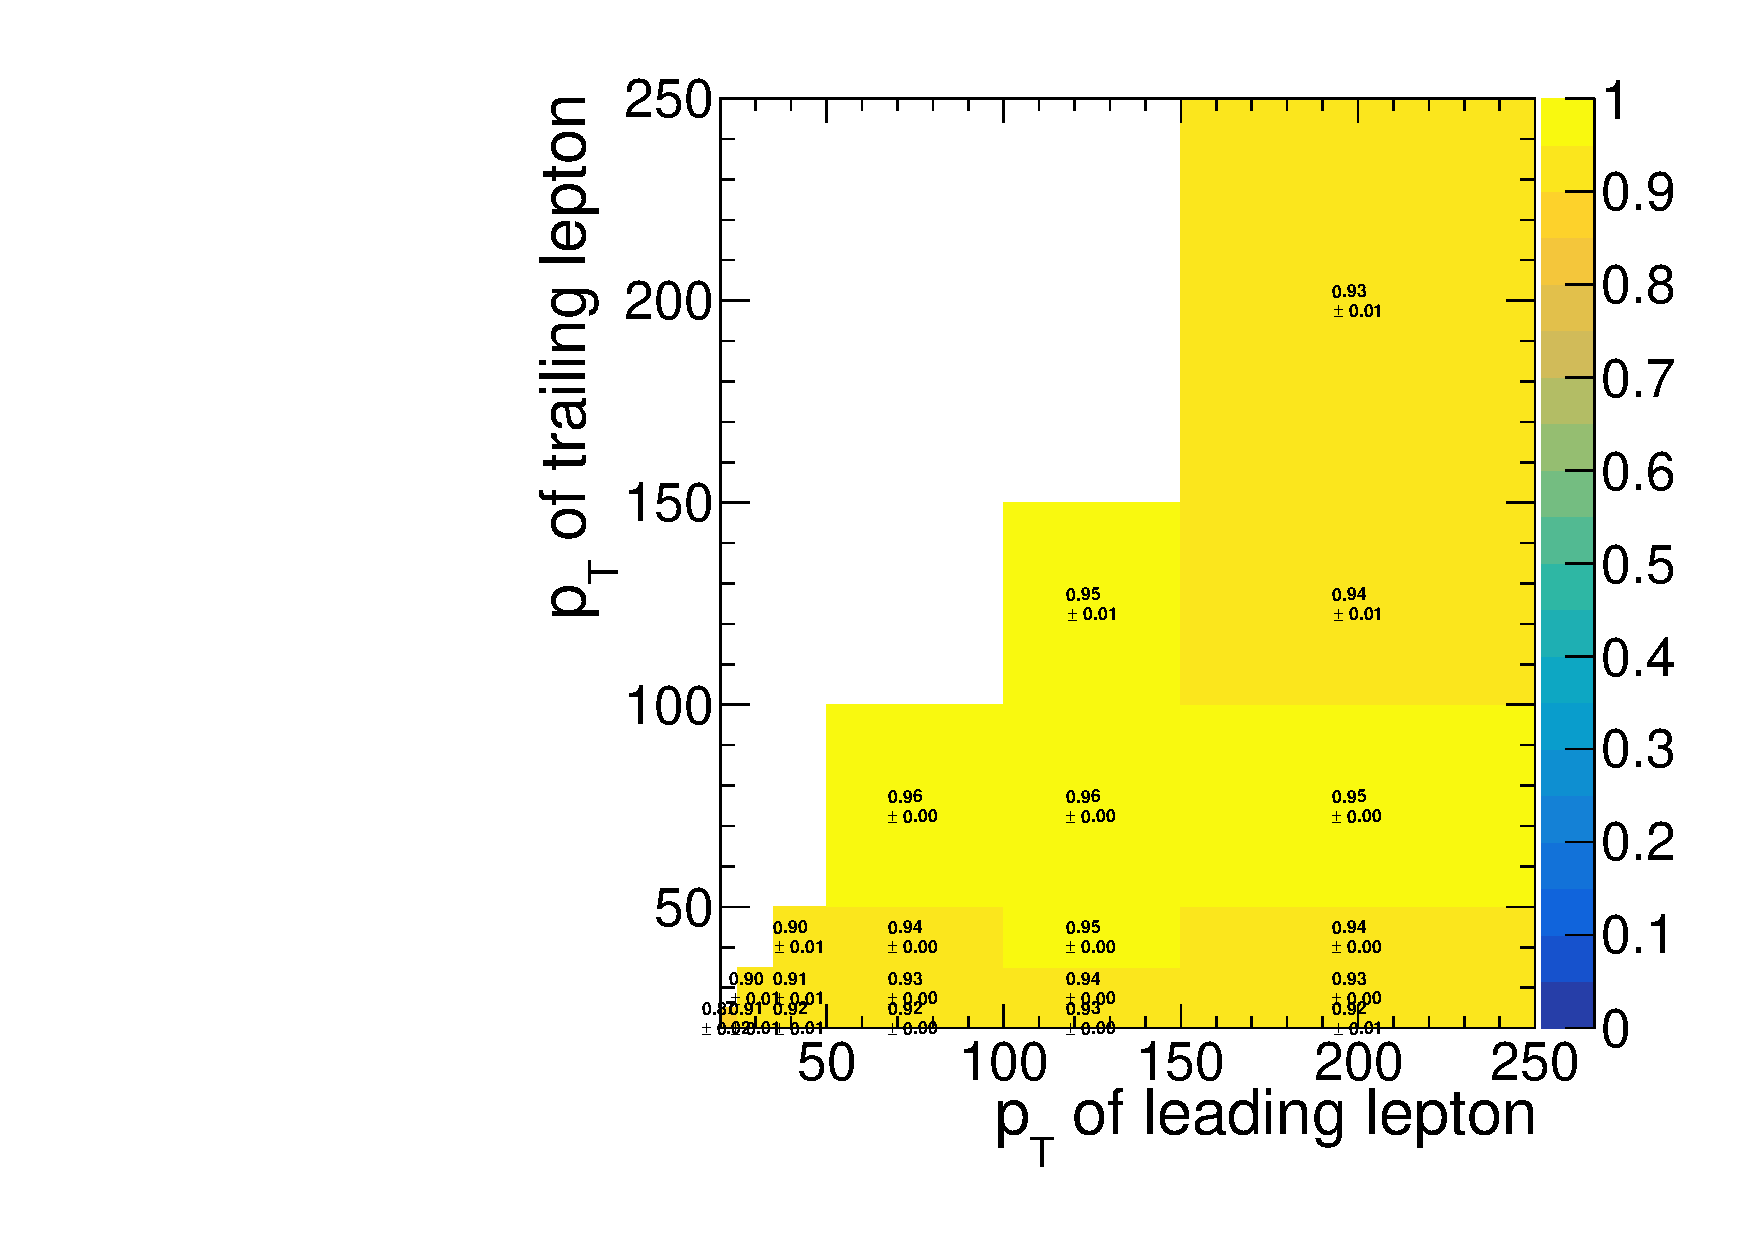
\includegraphics[width=0.5\textwidth]{figures/trigger/HLT_mumuIso_OR_HLT_mumuNoiso_OR_HLT_SingleMu_noniso_pt1_pt2_highEta1_veryCoarse_BCDEF.pdf}}
  \caption{Gain in trigger efficiency for the $\mu\mu$ channel by adding non-isolated and single-lepton triggers}
  \label{fig:additionalTriggers}
\end{figure}

We measure the trigger efficiencies in the unbiased {\verb MET } and {\verb JetHT } data sets which give consistent results. 
We use the measurement obtained in the {\verb MET } because of the smaller statistical uncertainties.
There is a significant inefficiency for muons with high transverse momentum in the muon endcaps, hence
we parametrize the trigger inefficiency as a function of the two lepton momenta and define two bins of the $\eta$ of the leading lepton that are separated by $|\eta|=1.5$. In the e$\mu$ channel, we bin the measurement in the same way but we take the $\eta$ of the muon, whether it is leading or not. 
The measured trigger efficiencies are used to scale the simulation.

Figure~\ref{fig:additionalTriggers} shows the gain in trigger efficiency by including the non-isolated double-lepton and, additionally, the single-lepton triggers for the example of the $\mu\mu$ channel and for $|\eta|>1.5$ for the leading muon. The improvement at high transverse momenta is dramatic. All other trigger efficiency maps show less prominent effects and are collected in Appendix~\ref{app:triggerEff}.
